\documentclass[11pt,a4paper]{article}

% --- Packages -----------------------------------------------------------------
\usepackage[margin=2.4cm]{geometry}
\usepackage[T1]{fontenc}
\usepackage[utf8]{inputenc}
\usepackage[scaled=0.92]{inconsolata}
\renewcommand{\familydefault}{\ttdefault}
\usepackage{graphicx}
\usepackage{booktabs}
\usepackage{tabularx}
\usepackage{hyperref}
\usepackage{xcolor}
\usepackage{listings}
\usepackage{tikz}
\usepackage{enumitem}
\usepackage{caption}
\usepackage{subcaption}
\usepackage{float}
\usepackage{fancyhdr}
\usepackage{titlesec}
\usepackage{csquotes}
\usepackage{amsmath}
\usetikzlibrary{arrows.meta,positioning,fit,calc,shapes.geometric,shapes.multipart}

\hypersetup{
  colorlinks=true,
  linkcolor=black!70!blue,
  urlcolor=black!70!blue,
  citecolor=black!70!blue,
  pdftitle={SURF Invite -- MidPoint Integration (MidPoint-leading)},
  pdfauthor={MidPoint Invite Integration}
}

\definecolor{codebg}{RGB}{246,246,248}
\definecolor{accent}{RGB}{36,87,214}
\definecolor{good}{RGB}{18,121,91}
\definecolor{muted}{RGB}{93,104,122}

\lstset{
  basicstyle=\ttfamily\footnotesize,
  backgroundcolor=\color{codebg},
  frame=single,
  framerule=0.3pt,
  rulecolor=\color{black!20},
  breaklines=true,
  columns=fullflexible,
  keepspaces=true,
  showstringspaces=false,
  xleftmargin=0.5em,
  xrightmargin=0.5em,
  aboveskip=0.8em,
  belowskip=0.8em
}

\pagestyle{fancy}
\fancyhf{}
\fancyhead[L]{\small MidPoint Invite Integration}
\fancyhead[R]{\small SURF Demo}
\fancyfoot[C]{\thepage}
\renewcommand{\headrulewidth}{0.3pt}

\titleformat{\section}{\Large\bfseries\color{accent}}{\thesection}{0.8em}{}
\titleformat{\subsection}{\large\bfseries}{\thesubsection}{0.7em}{}

\newcommand{\host}[1]{\texttt{#1}}
\newcommand{\svc}[1]{\texttt{#1}}

% --- Document -----------------------------------------------------------------
\title{%
  SURF Invite -- MidPoint Integration\\
  \large MidPoint-leading reference architecture and operator guide
}
\author{Reference implementation\\(\texttt{midpoint-invite-integration}, branch \texttt{midpoint-leading})}
\date{\today}

\begin{document}
\maketitle

\begin{abstract}
This document describes a reference stack that integrates
\textbf{SURFconext Invite} with \textbf{MidPoint}.
\textbf{MidPoint is the system of record for roles/groups}: an
\texttt{invite\_bridge} service creates and deletes matching Roles in Invite
via the Invite external API, and notifies Invite when a MidPoint administrator
unassigns an Invite-provisioned membership (\texttt{by\_provisioned\_scim}) so
VOOT/AA and app access do not drift.
\textbf{Invite} remains the invitation UX (and may be started from MidPoint via
an \textbf{Invite user} menu link); after a guest accepts, Invite provisions
\textbf{users and memberships} into MidPoint over institutional
\textbf{SCIM~2.0}.
An optional OIDC demo application is included for verification; Moodle and
OpenLDAP are parked (code retained, not in the default compose).
\end{abstract}

\tableofcontents
\newpage

% =============================================================================
\section{Goals and design rationale}
% =============================================================================

The reference answers three practical questions:

\begin{enumerate}[leftmargin=*]
  \item How can an institution create roles in \textbf{MidPoint} and have them
        appear automatically in \textbf{SURF Invite} for invitation workflows?
  \item How can a MidPoint administrator \textbf{invite a guest} without leaving
        MidPoint, while still using Invite's invitation email and accept flow?
  \item How do invited guests still land in MidPoint as users with role
        assignments via \textbf{SCIM}, without Invite creating duplicate Roles?
  \item How does MidPoint notify Invite when an administrator \textbf{revokes}
        an Invite-provisioned membership (drift prevention)?
  \item What minimal custom code must another MidPoint deployment reuse
        (\texttt{invite\_bridge} + SCIM MidPoint plugin leading mode)?
\end{enumerate}

\paragraph{Core principle.}
MidPoint owns the Role lifecycle (create/delete). Invite owns inviting and
accepting guests. SCIM carries Users and memberships from Invite into MidPoint.
When Invite echoes a SCIM Group create after the bridge created the Invite Role,
the SCIM MidPoint plugin (\texttt{MIDPOINT\_LEADING\_GROUPS}) matches the
existing Role by name and does not create a second Role.
When a MidPoint admin unassigns an Invite-SCIM user from an Invite-SCIM role,
\texttt{invite\_bridge} calls Invite
\texttt{DELETE \ldots/user\_roles/by\_provisioned\_scim/\{userScimId\}/\{groupScimId\}}.

% =============================================================================
\section{System overview}
% =============================================================================

\subsection{Components}

\begin{table}[H]
\centering
\begin{tabularx}{\textwidth}{@{}l X l@{}}
\toprule
\textbf{Component} & \textbf{Role} & \textbf{Hostname (Traefik)} \\
\midrule
MidPoint + Postgres & IDM/IGA; SoR for Roles; users, assignments &
  \host{midpoint.\$DOMAIN} \\
\texttt{invite\_bridge} & MidPoint Roles $\leftrightarrow$ Invite API;
  membership revoke notify; \textbf{Invite user} form &
  \host{invite-bridge.\$DOMAIN} \\
SURF Invite & Invitation UX; SCIM client for Users/memberships & (external) \\
SCIM service & Institutional SCIM API $\rightarrow$ MidPoint REST &
  \host{scim.\$DOMAIN} \\
OIDC Application & Optional membership-pull demo &
  \host{app.\$DOMAIN} \\
SURFconext / eduID & OIDC authentication & (external) \\
\bottomrule
\end{tabularx}
\caption{Stack components and Traefik hostnames (default compose).
  Moodle and OpenLDAP are parked---see Section~\ref{sec:parked}.}
\end{table}

\subsection{Logical architecture}

\begin{figure}[H]
\centering
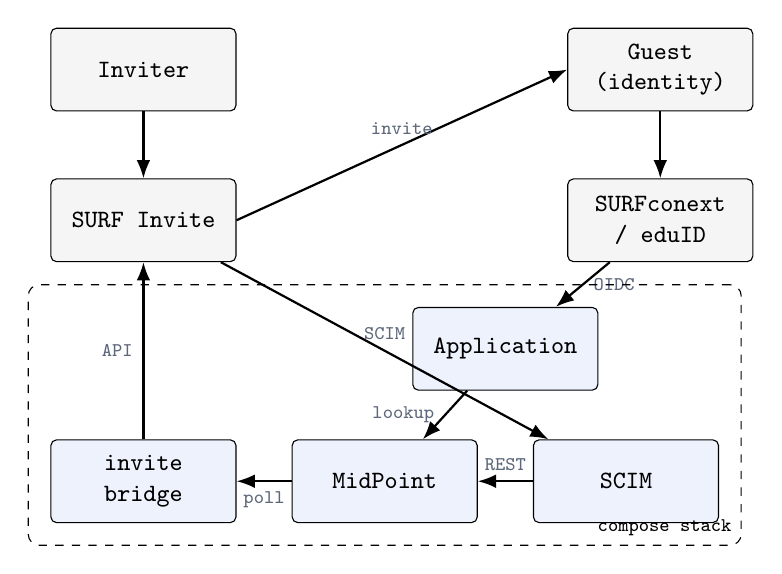
\begin{tikzpicture}[
  font=\small\ttfamily,
  box/.style={draw, rounded corners=2pt, align=center, inner sep=5pt, minimum height=1.05cm, minimum width=2.35cm},
  ext/.style={box, fill=black!4},
  int/.style={box, fill=accent!8},
  arr/.style={-Latex, thick},
  note/.style={font=\scriptsize\ttfamily, text=muted}
]
  % Actors
  \node[ext] (inviter) {Inviter};
  \node[ext, right=4.2cm of inviter] (guest) {Guest\\(identity)};

  % External services
  \node[ext, below=0.85cm of inviter] (invite) {SURF Invite};
  \node[ext, below=0.85cm of guest] (op) {SURFconext\\/ eduID};

  % Compose stack
  \node[int, below=2.25cm of invite] (bridge) {invite\\bridge};
  \node[int, right=0.7cm of bridge] (mp) {MidPoint};
  \node[int, right=0.7cm of mp] (scim) {SCIM};

  \node[int, above=1.15cm of $(mp)!0.5!(scim)$] (app) {Application};

  \draw[arr] (inviter) -- (invite);
  \draw[arr] (invite.east) -- node[above,note]{invite} (guest.west);
  \draw[arr] (mp) -- node[below,note]{poll} (bridge);
  \draw[arr] (bridge) -- node[left,note]{API} (invite);
  \draw[arr] (invite) -- node[above,note]{SCIM} (scim);
  \draw[arr] (scim) -- node[above,note]{REST} (mp);
  \draw[arr] (guest) -- (op);
  \draw[arr] (op) -- node[right,note]{OIDC} (app);
  \draw[arr] (app) -- node[left,note]{lookup} (mp);

  \node[draw, dashed, rounded corners=4pt, fit=(bridge)(mp)(scim)(app),
        inner sep=8pt, label={[anchor=south east,font=\scriptsize\ttfamily]south east:compose stack}] {};
\end{tikzpicture}
\caption{Logical architecture (MidPoint-leading).
Roles and membership revokes flow MidPoint $\rightarrow$ Invite via
\texttt{invite\_bridge}; users/memberships flow
Invite $\rightarrow$ SCIM $\rightarrow$ MidPoint.
The OIDC app is an optional demo target.}
\label{fig:architecture}
\end{figure}

\subsection{Repository layout}

\begin{lstlisting}
compose.yml / compose.traefik.yml / Makefile
invite_bridge/                 # Roles <-> Invite + revoke notify + form
scripts/invite-create-role.sh
scripts/integration_membership_revoke.py
application/                   # OIDC membership-pull demo (optional)
midpoint/post-initial-objects/ # scimResource schema (+ parked LDAP XML)
docs/latex/                    # this operator guide
docs/scim-curl.md
design.puml                    # MidPoint-leading sequence
\end{lstlisting}

% =============================================================================
\section{MidPoint-leading provisioning flow}
% =============================================================================

MidPoint owns Role create/delete. Invite owns invitations.
Figure~\ref{fig:invite-sequence} shows the sequence (from \texttt{design.puml};
regenerate the PNG after editing the PlantUML source).

\begin{figure}[H]
\centering
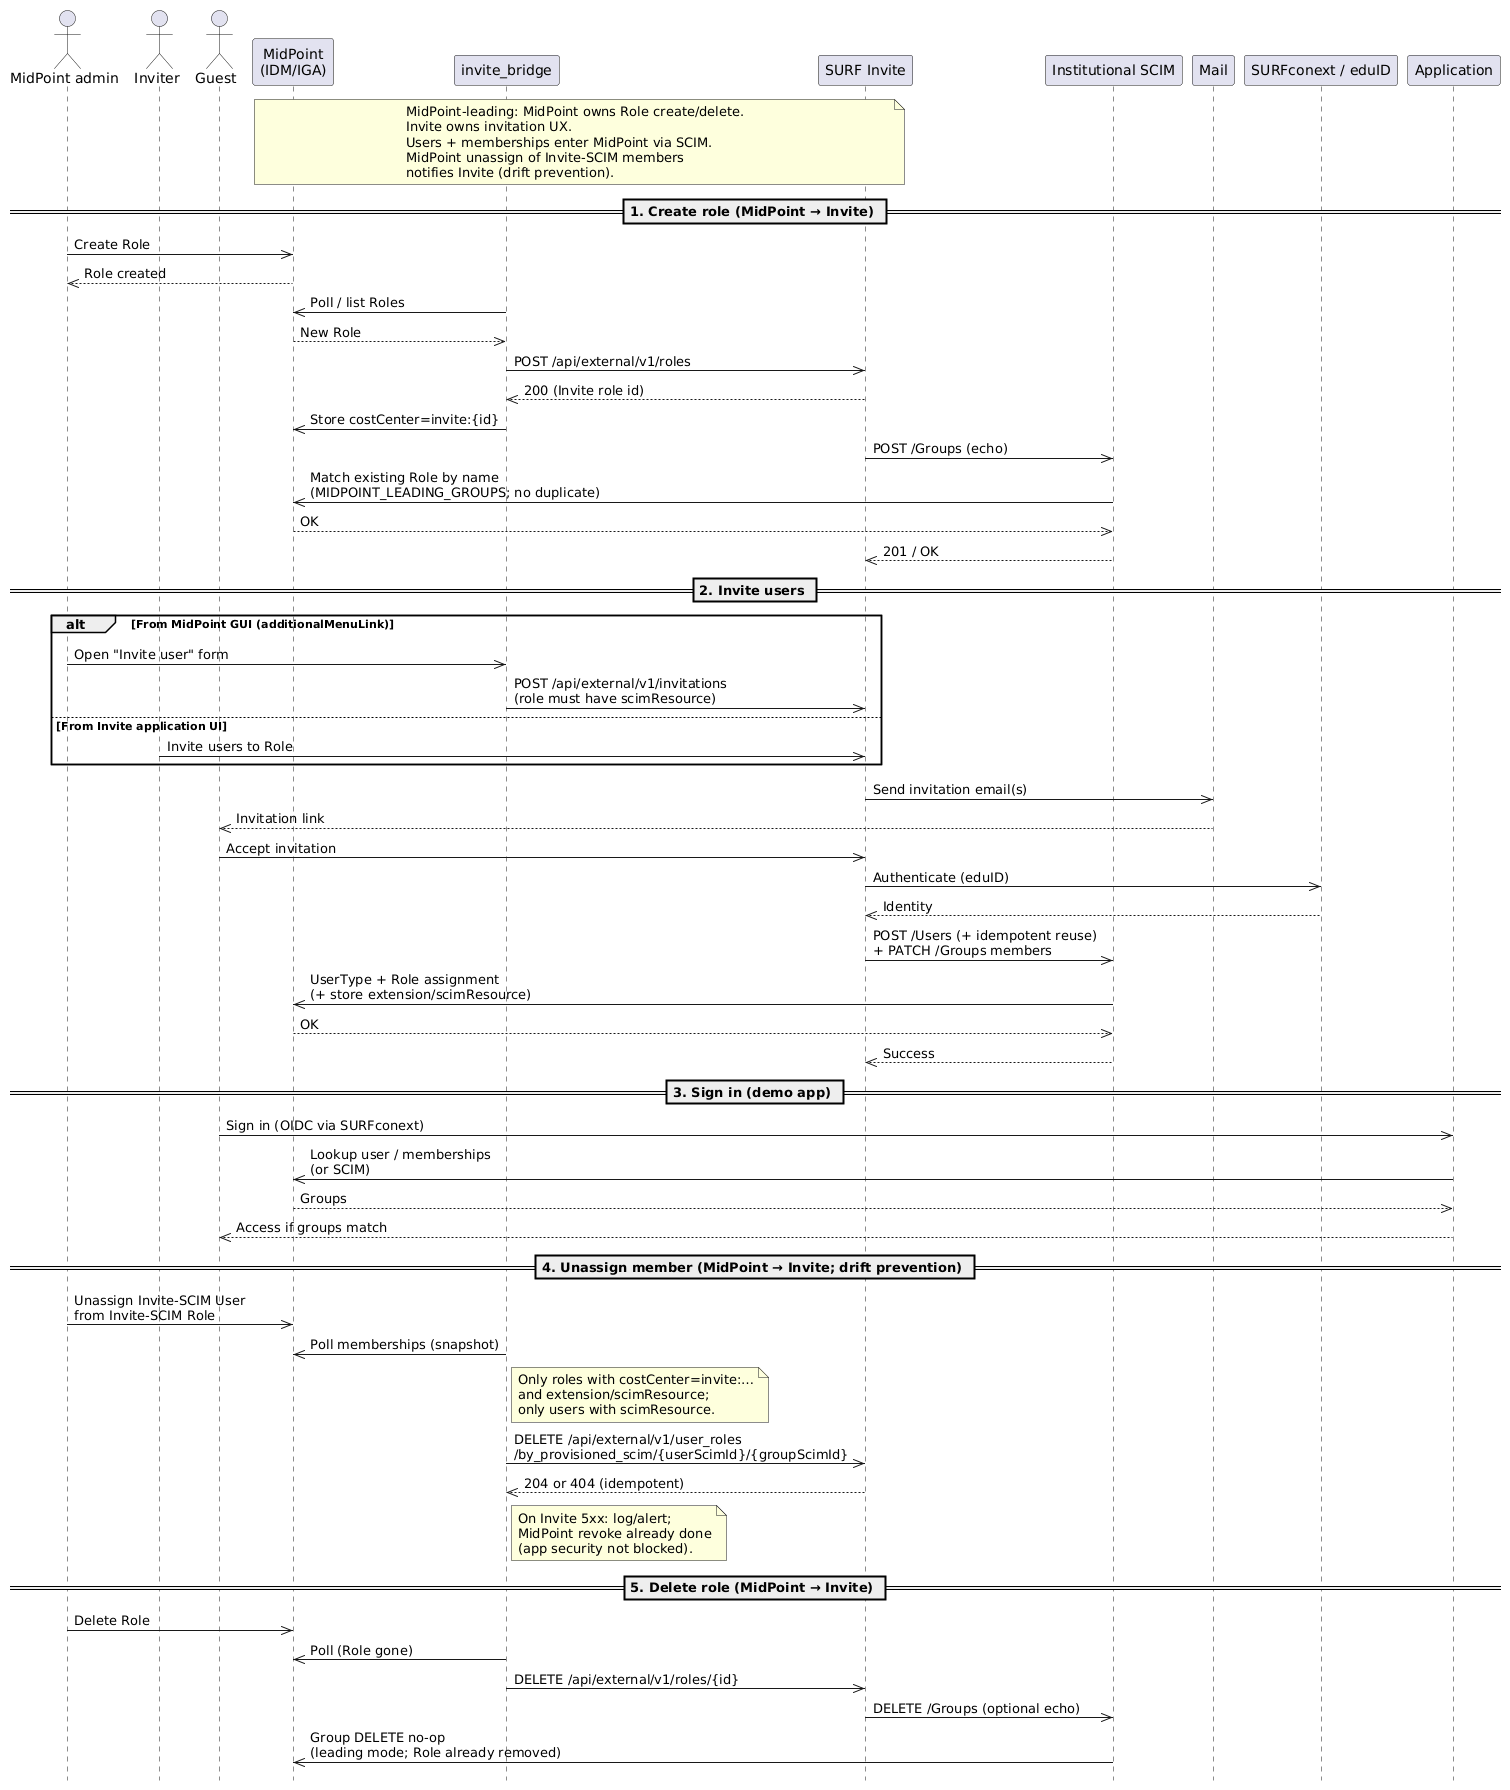
\includegraphics[width=\textwidth]{figures/invite-sequence.png}
\caption{MidPoint-leading sequence: create Role, invite guest, sign-in,
  unassign member (drift prevention), delete Role.}
\label{fig:invite-sequence}
\end{figure}

\subsection{SURF Invite provisioner configuration}
\label{sec:invite-provisioner}

Before Invite can drive MidPoint, the institutional SCIM endpoint must be
registered as a \emph{provisioning} service in SURF Conext Manage.
Figure~\ref{fig:manage-provisioner} shows the metadata used for this demo.

\begin{figure}[H]
\centering
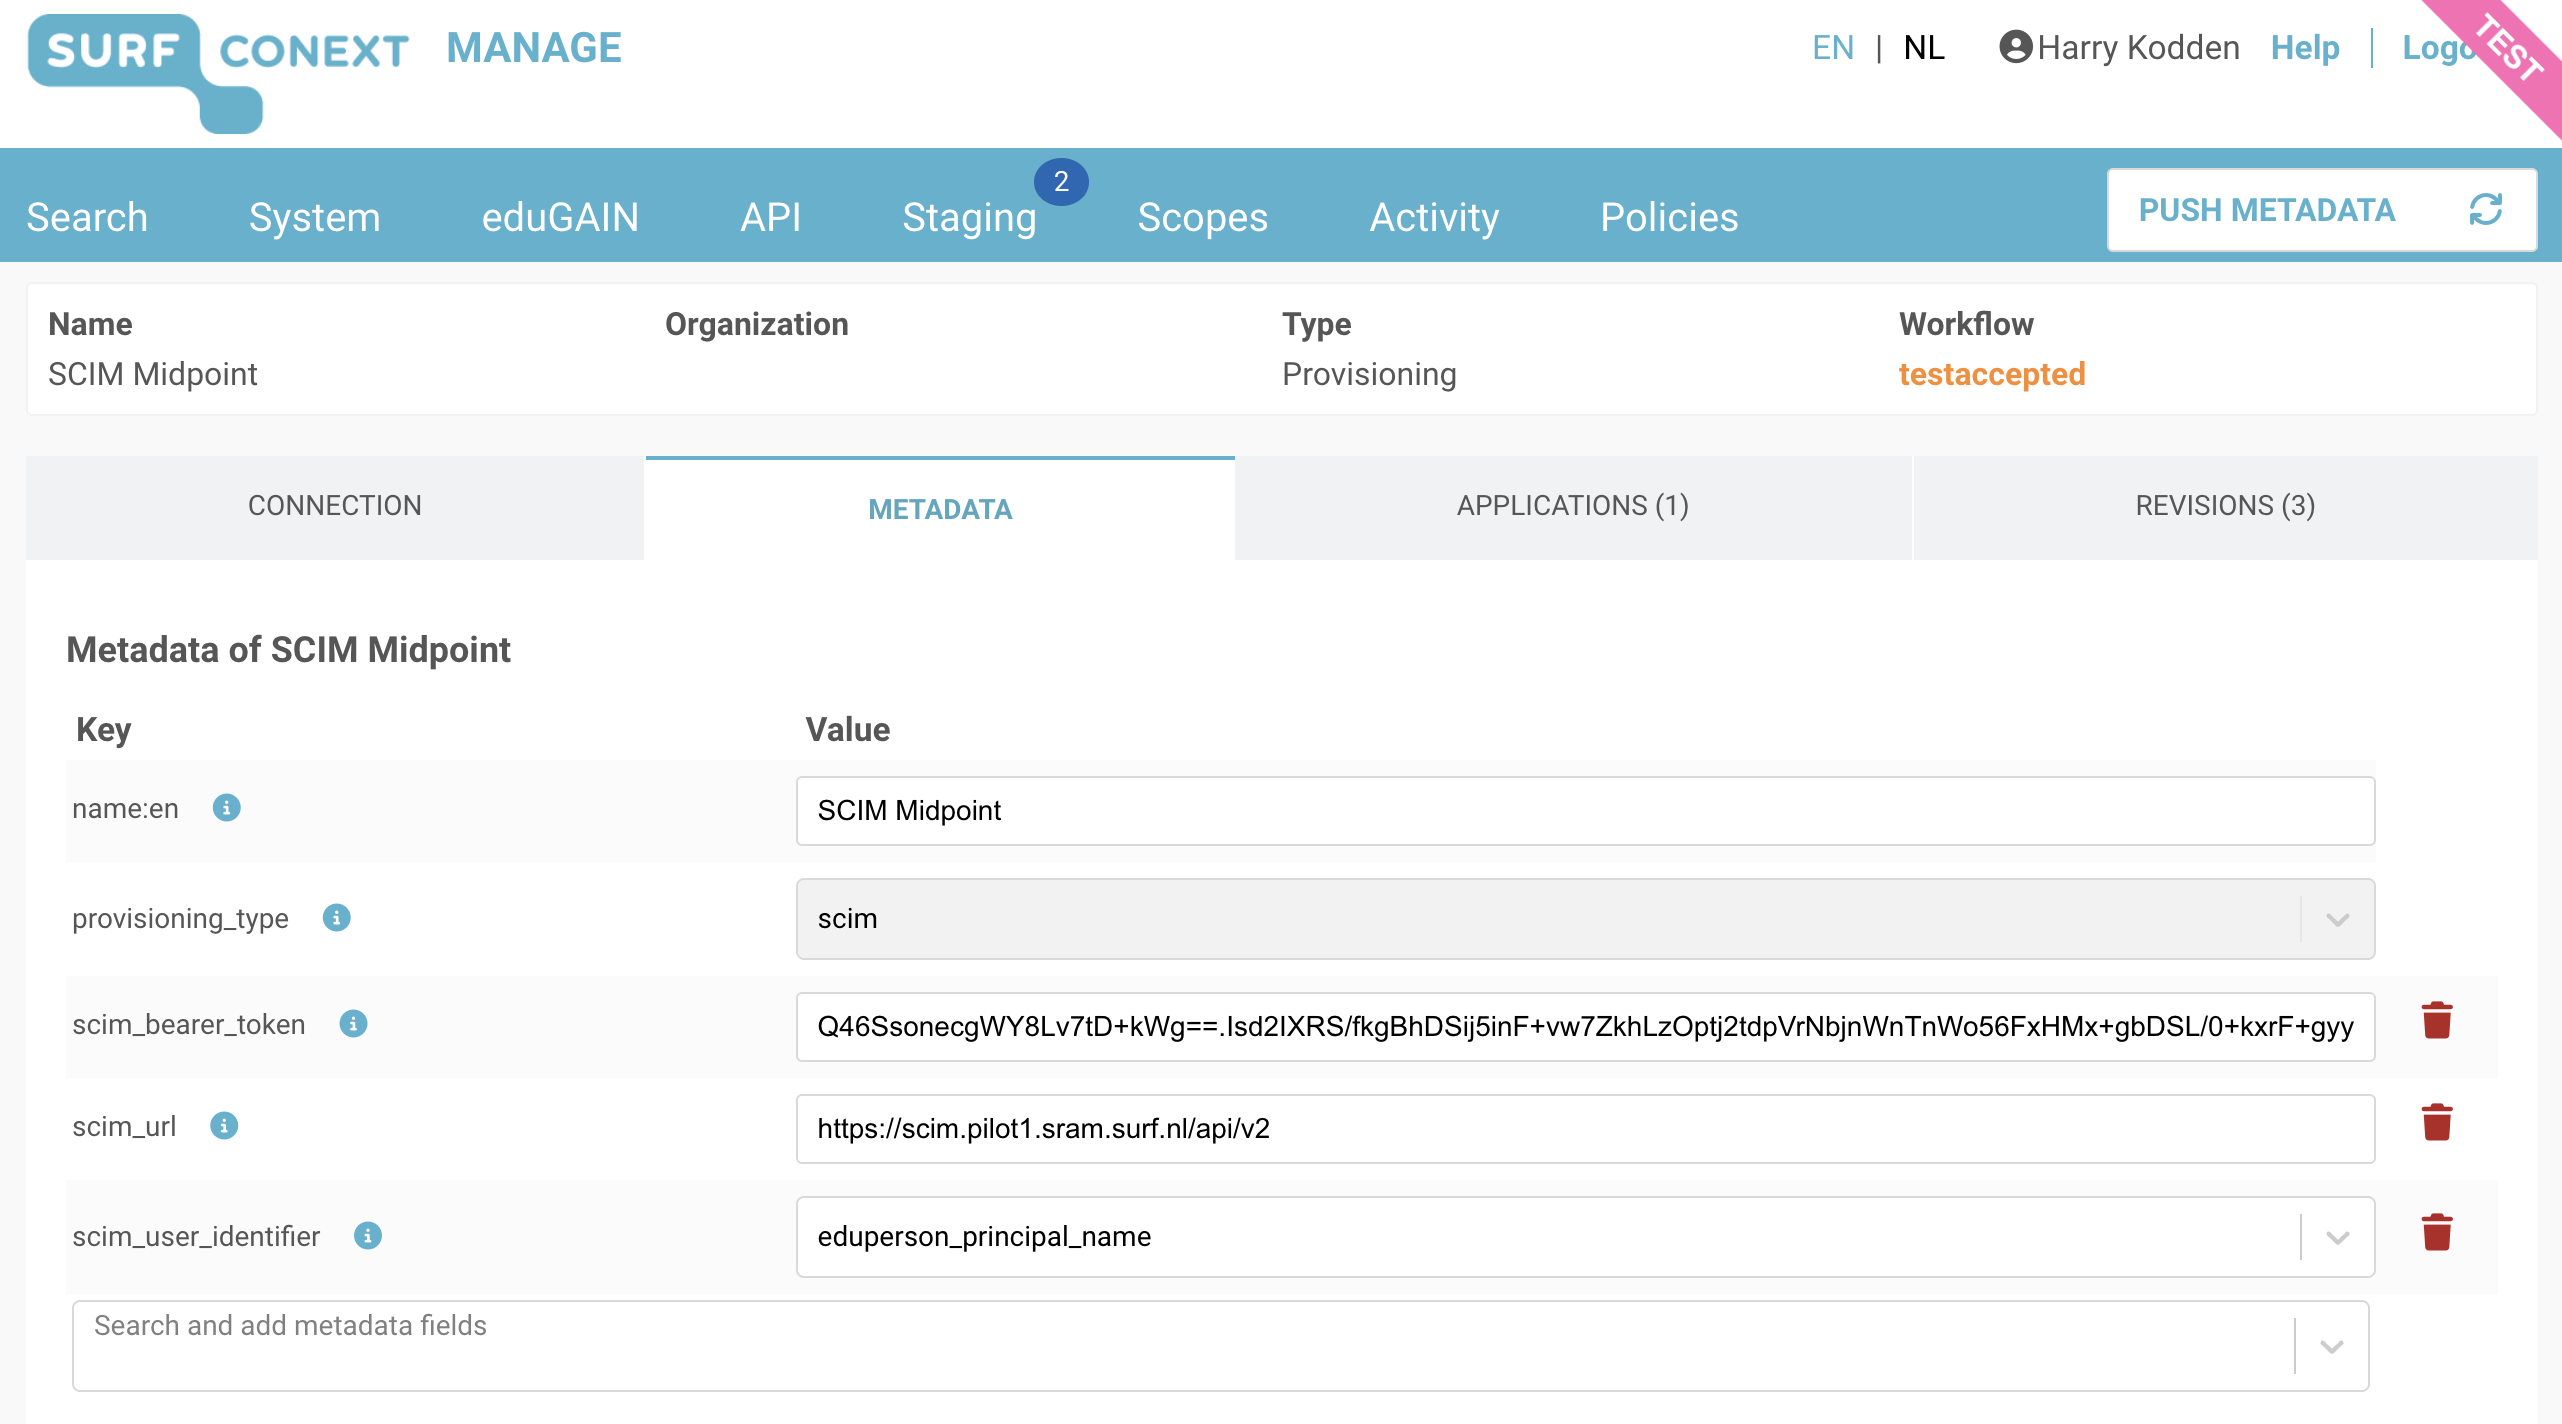
\includegraphics[width=\textwidth]{figures/manage-provisioner.png}
\caption{SURF Conext Manage: metadata for the \texttt{SCIM Midpoint} provisioning
  service (type \texttt{scim}), pointing at the demo SCIM base URL and using
  \texttt{eduperson\_principal\_name} as the user identifier.}
\label{fig:manage-provisioner}
\end{figure}

The essential fields are:

\begin{description}[style=nextline,leftmargin=1.2em]
  \item[\texttt{provisioning\_type}]
    Set to \texttt{scim} so Invite pushes Users/Groups over SCIM~2.0.
  \item[\texttt{scim\_url}]
    Base URL of the institutional SCIM API, including the path prefix
    (here \texttt{https://scim.pilot1.sram.surf.nl/api/v2}).
  \item[\texttt{scim\_bearer\_token}]
    Shared secret presented as an HTTP Bearer token; must match
    \texttt{SCIM\_API\_KEY} in the compose stack.
  \item[\texttt{scim\_user\_identifier}]
    Claim used to correlate Invite guests with SCIM/MidPoint users
    (\texttt{eduperson\_principal\_name} in this setup---the same key the
    demo application uses via \texttt{USER\_LOOKUP\_CLAIMS}).
\end{description}

With this metadata in place (and Invite using \emph{remote} Manage, not static
seed apps), Invite can push Users/memberships (and Group echoes) to SCIM.

\subsection{Detailed steps}

\begin{description}[style=nextline,leftmargin=1.2em]
  \item[1. Create role (MidPoint-leading)]
    MidPoint administrator creates an application Role.
    \texttt{invite\_bridge} polls MidPoint and calls Invite
    \texttt{POST /api/external/v1/roles}, then stores
    \texttt{costCenter=invite:\{id\}} on the MidPoint Role.
    Invite may echo \texttt{POST /Groups} to SCIM; with
    \texttt{MIDPOINT\_LEADING\_GROUPS} the plugin reuses the existing Role by
    name (no duplicate).
  \item[2. Invite and accept]
    An invitation can be started either in the \textbf{Invite application UI} or
    from MidPoint via the \textbf{Invite user} menu (Section~\ref{sec:invite-user-ui}).
    After eduID authentication, Invite issues SCIM User create/update and Group
    membership changes. SCIM creates/updates MidPoint \texttt{UserType} and role
    assignments, and stores the raw SCIM document on
    \texttt{extension/scimResource}.
    With \texttt{SCIM\_IDEMPOTENT\_USER\_CREATE}, a re-\texttt{POST} for an
    existing \texttt{userName}/\texttt{externalId} reuses the User (no 409).
  \item[3. Application sign-in]
    Guest authenticates to the demo application via SURFconext/eduID (OIDC).
    The application resolves the lookup key (e.g.\
    \texttt{eduperson\_principal\_name}) and evaluates memberships via MidPoint
    or SCIM.
  \item[4. Unassign member (drift prevention)]
    When a MidPoint admin removes an Invite-SCIM user from an Invite-SCIM role,
    \texttt{invite\_bridge} calls
    \texttt{DELETE /api/external/v1/user\_roles/by\_provisioned\_scim/\{userScimId\}/\{groupScimId\}}
    using MidPoint's SCIM resource ids. Invite \texttt{404} is treated as
    success; other Invite errors are logged while MidPoint revoke stands.
  \item[5. Delete role]
    Deleting the MidPoint Role causes \texttt{invite\_bridge} to
    \texttt{DELETE} the Invite Role. Invite-initiated membership remove still
    flows over SCIM into MidPoint.
\end{description}

\subsection{Reusable custom code}

\begin{description}[style=nextline,leftmargin=1.2em]
  \item[\texttt{invite\_bridge/}]
    Python service: MidPoint Role create/delete $\leftrightarrow$ Invite
    external API; membership revoke $\rightarrow$
    \texttt{by\_provisioned\_scim}; Invite-user form. Required for
    MidPoint-leading.
  \item[SCIM MidPoint plugin]
    Sibling \texttt{scim} checkout; set \texttt{MIDPOINT\_LEADING\_GROUPS=true}
    so Invite Group echoes do not create or delete MidPoint Roles incorrectly.
    Prefer \texttt{SCIM\_IDEMPOTENT\_USER\_CREATE=true} for Invite re-provision.
\end{description}

\subsection{SCIM $\leftrightarrow$ MidPoint mapping}

\begin{table}[H]
\centering
\begin{tabularx}{\textwidth}{@{}l X X@{}}
\toprule
\textbf{SCIM} & \textbf{MidPoint} & \textbf{Notes} \\
\midrule
Users & \texttt{UserType} &
  \texttt{userName}$\rightarrow$\texttt{name},
  \texttt{displayName}$\rightarrow$\texttt{fullName} \\
Groups & \texttt{RoleType} &
  \texttt{displayName}$\rightarrow$\texttt{name}/\texttt{displayName} \\
Group members & User \texttt{assignment} &
  \texttt{targetRef} to \texttt{RoleType} \\
SCIM document & \texttt{extension/scimResource}
  (legacy: \texttt{description}) &
  Hidden schema-extension attribute; marks Invite-provisioned objects \\
\bottomrule
\end{tabularx}
\caption{SCIM MidPoint plugin mapping used by this stack.}
\end{table}

% =============================================================================
\section{Invite user from MidPoint}
\label{sec:invite-user-ui}
% =============================================================================

MidPoint administrators can start an Invite invitation without switching to the
Invite application. The \texttt{invite\_bridge} service:

\begin{enumerate}[leftmargin=*]
  \item Serves a small HTML form at
        \host{https://invite-bridge.\$DOMAIN/invite}
        (HTTP Basic auth in this demo).
  \item On startup, registers a MidPoint
        \texttt{adminGuiConfiguration/additionalMenuLink} labelled
        \textbf{Invite user} that points at that URL.
  \item On submit, calls Invite \texttt{POST /api/external/v1/invitations}
        (email + Invite role id). \textbf{No MidPoint User is created} until the
        guest accepts and Invite provisions via SCIM.
\end{enumerate}

\paragraph{Role eligibility.}
The form lists only MidPoint Roles that Invite has already SCIM-provisioned
(they carry \texttt{extension/scimResource}, or legacy SCIM JSON in
\texttt{description}) and that have an Invite role id
(\texttt{costCenter=invite:\{id\}}). Roles that exist only in MidPoint, or only
in Invite without a SCIM echo, are omitted.

\begin{figure}[H]
\centering
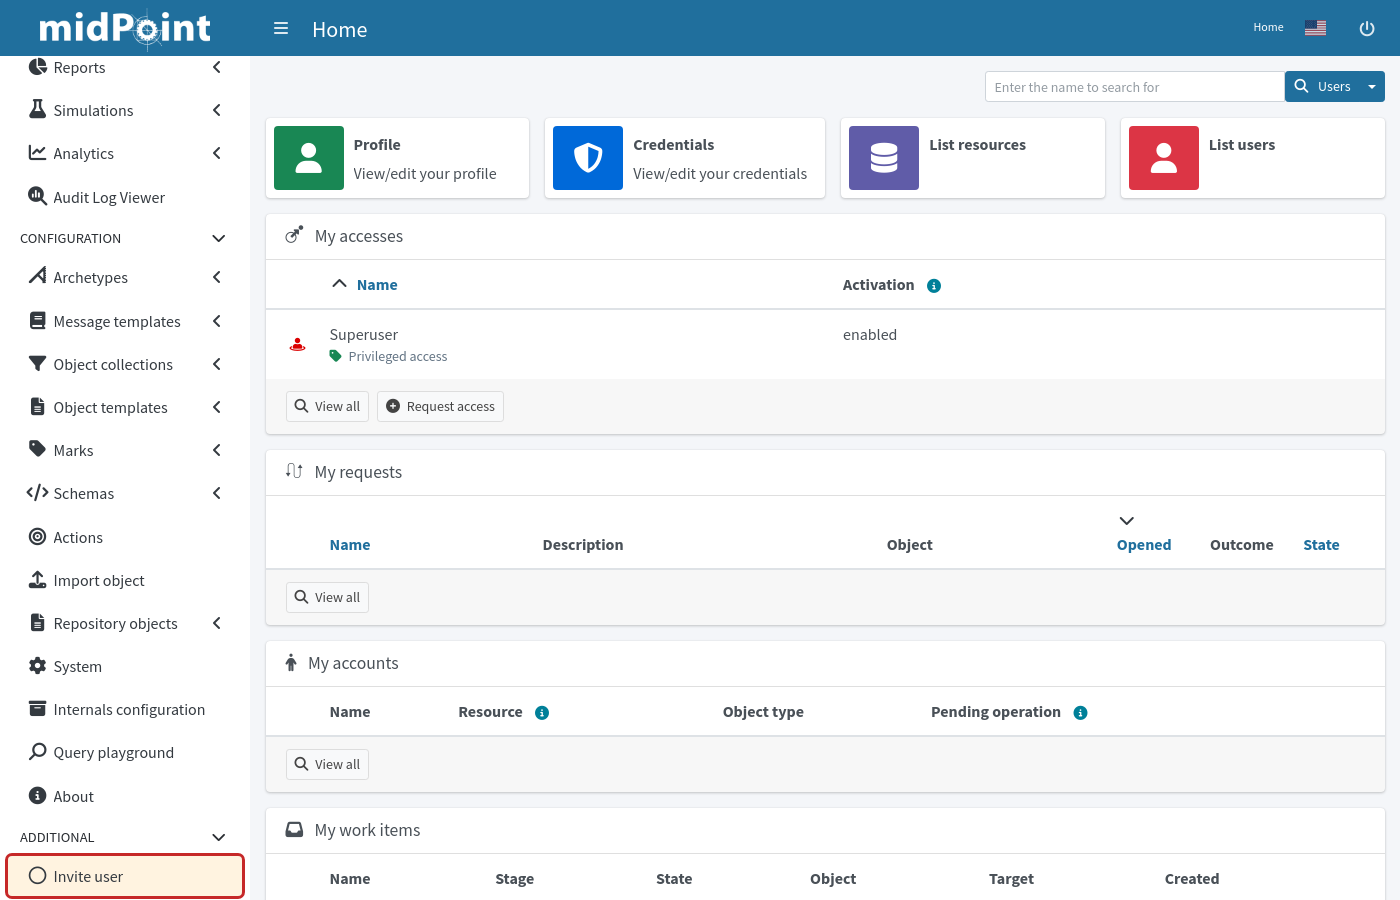
\includegraphics[width=0.95\textwidth]{figures/midpoint-invite-menu.png}
\caption{MidPoint GUI: \textbf{Invite user} under the \emph{ADDITIONAL} menu
  (registered by \texttt{invite\_bridge} as \texttt{additionalMenuLink}).}
\label{fig:midpoint-invite-menu}
\end{figure}

\begin{figure}[H]
\centering
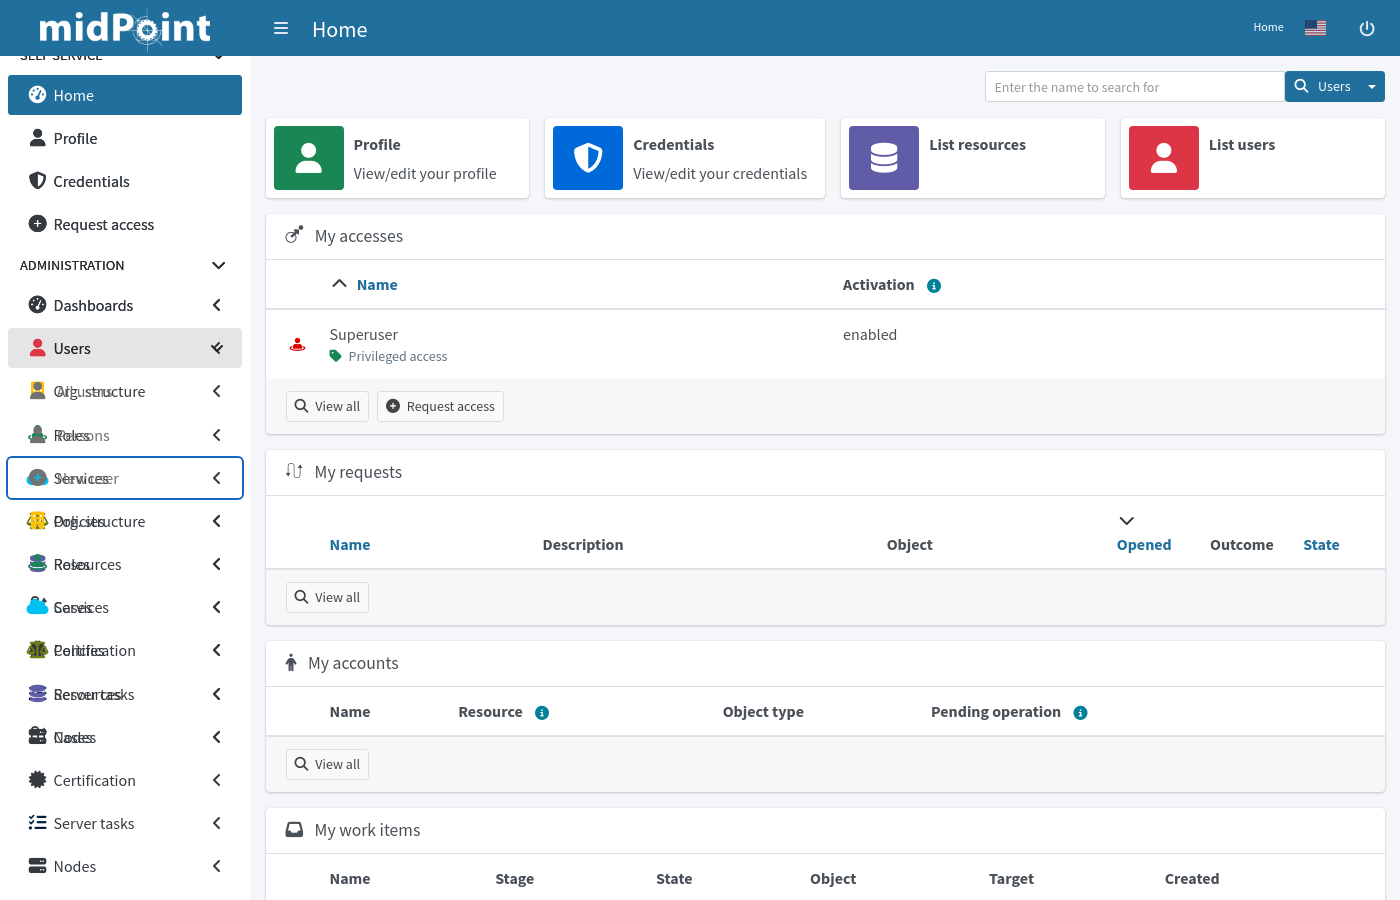
\includegraphics[width=0.72\textwidth]{figures/midpoint-users-menu.png}
\caption{For comparison: MidPoint \textbf{Users} menu still offers
  \textbf{New user} (creates a MidPoint \texttt{UserType} immediately).
  \textbf{Invite user} is a separate path that only creates an Invite invitation.}
\label{fig:midpoint-users-menu}
\end{figure}

\begin{figure}[H]
\centering
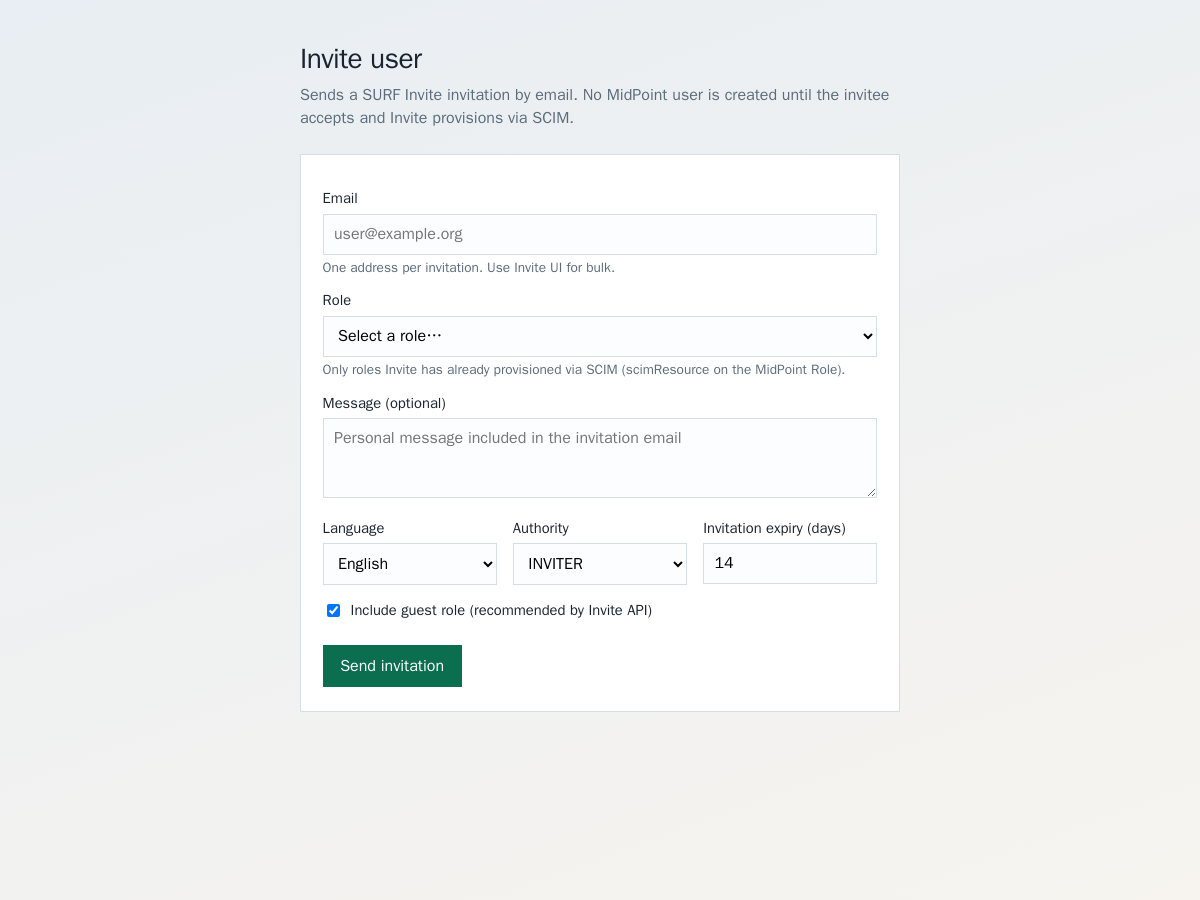
\includegraphics[width=0.88\textwidth]{figures/invite-user-form.png}
\caption{Invite user form served by \texttt{invite\_bridge}: email, SCIM-eligible
  role, optional message, language, authority, and expiry.
  Submitting calls Invite \texttt{POST /invitations}.}
\label{fig:invite-user-form}
\end{figure}

% =============================================================================
\section{OIDC application (membership pull)}
% =============================================================================

The demo application at \host{app.\$DOMAIN} is intentionally a \emph{pull}
authorization client. It is useful to verify what MidPoint/SCIM currently
know about a user.

\subsection{Operator flow}

\begin{enumerate}[leftmargin=*]
  \item \textbf{Select lookup method:} MidPoint or SCIM
        (LDAP remains in the app code for parked stacks).
  \item \textbf{Select required groups} listed by that backend.
  \item \textbf{Login with OIDC} (SURFconext). After callback, resolve the user
        key from \texttt{USER\_LOOKUP\_CLAIMS} and fetch memberships with the
        same backend. Access is granted when selected $\cap$ resolved is
        non-empty.
\end{enumerate}

\begin{figure}[H]
\centering
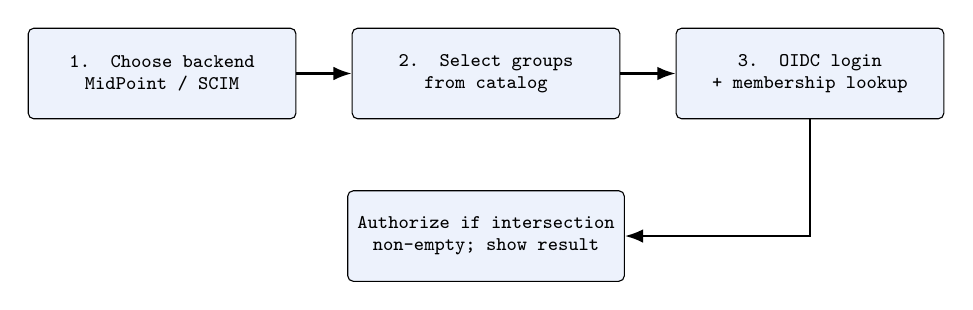
\begin{tikzpicture}[
  font=\scriptsize\ttfamily,
  stepbox/.style={draw, rounded corners=2pt, align=center, fill=accent!8,
               minimum width=3.4cm, minimum height=1.15cm},
  arr/.style={-Latex, thick}
]
  \node[stepbox] (s1) {1. Choose backend\\MidPoint / SCIM};
  \node[stepbox, right=0.7cm of s1] (s2) {2. Select groups\\from catalog};
  \node[stepbox, right=0.7cm of s2] (s3) {3. OIDC login\\+ membership lookup};
  \node[stepbox, below=0.9cm of s2] (s4) {Authorize if intersection\\non-empty; show result};
  \draw[arr] (s1) -- (s2);
  \draw[arr] (s2) -- (s3);
  \draw[arr] (s3) |- (s4);
\end{tikzpicture}
\caption{Application authorization wizard.}
\label{fig:app-flow}
\end{figure}

\subsection{Screenshots}

\begin{figure}[H]
\centering
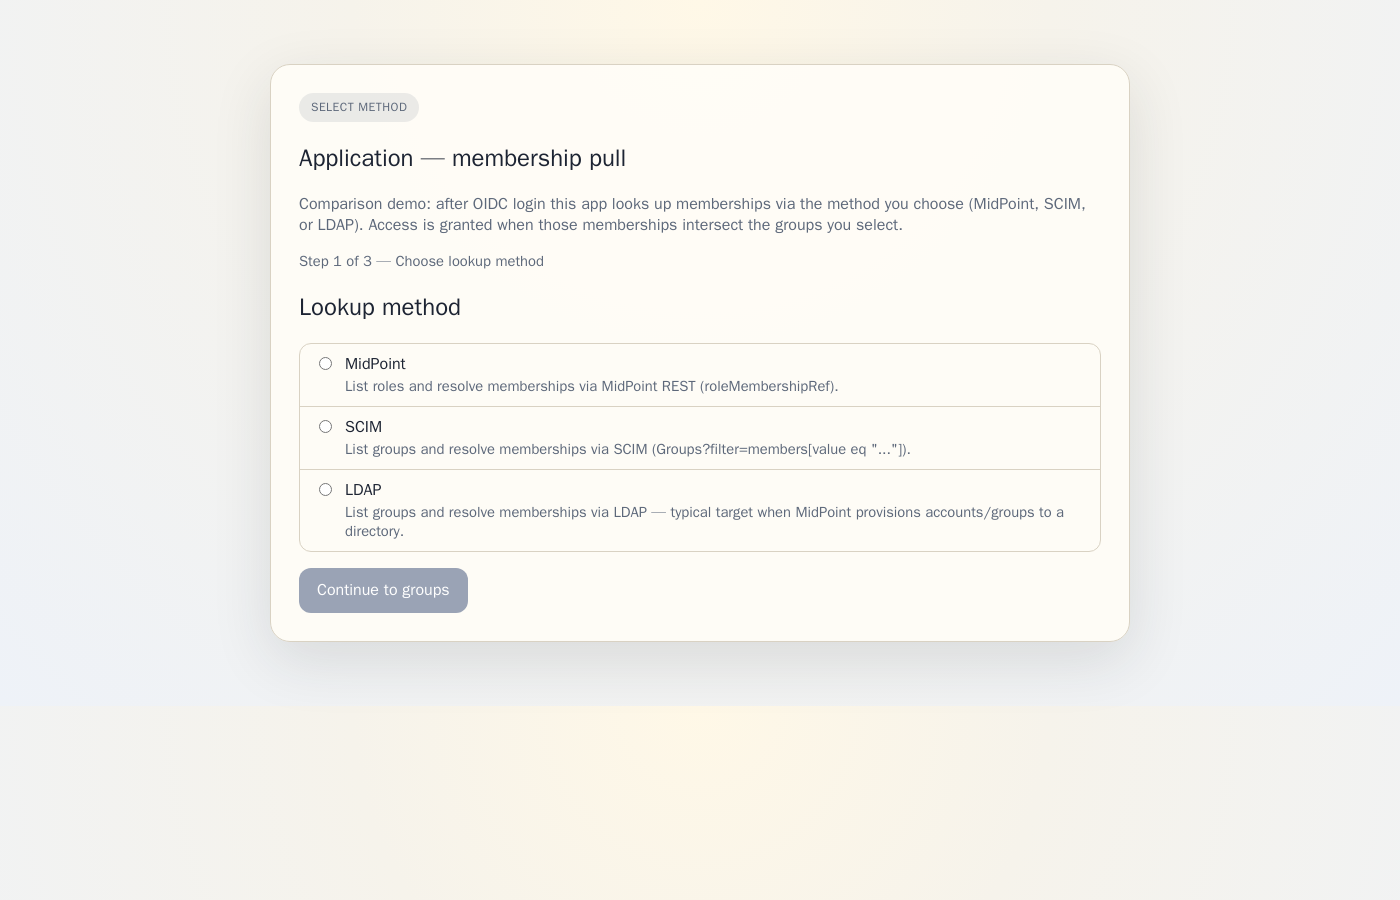
\includegraphics[width=0.92\textwidth]{figures/app-home.png}
\caption{Application --- Step 1: choose membership lookup backend.}
\label{fig:app-home}
\end{figure}

\begin{figure}[H]
\centering
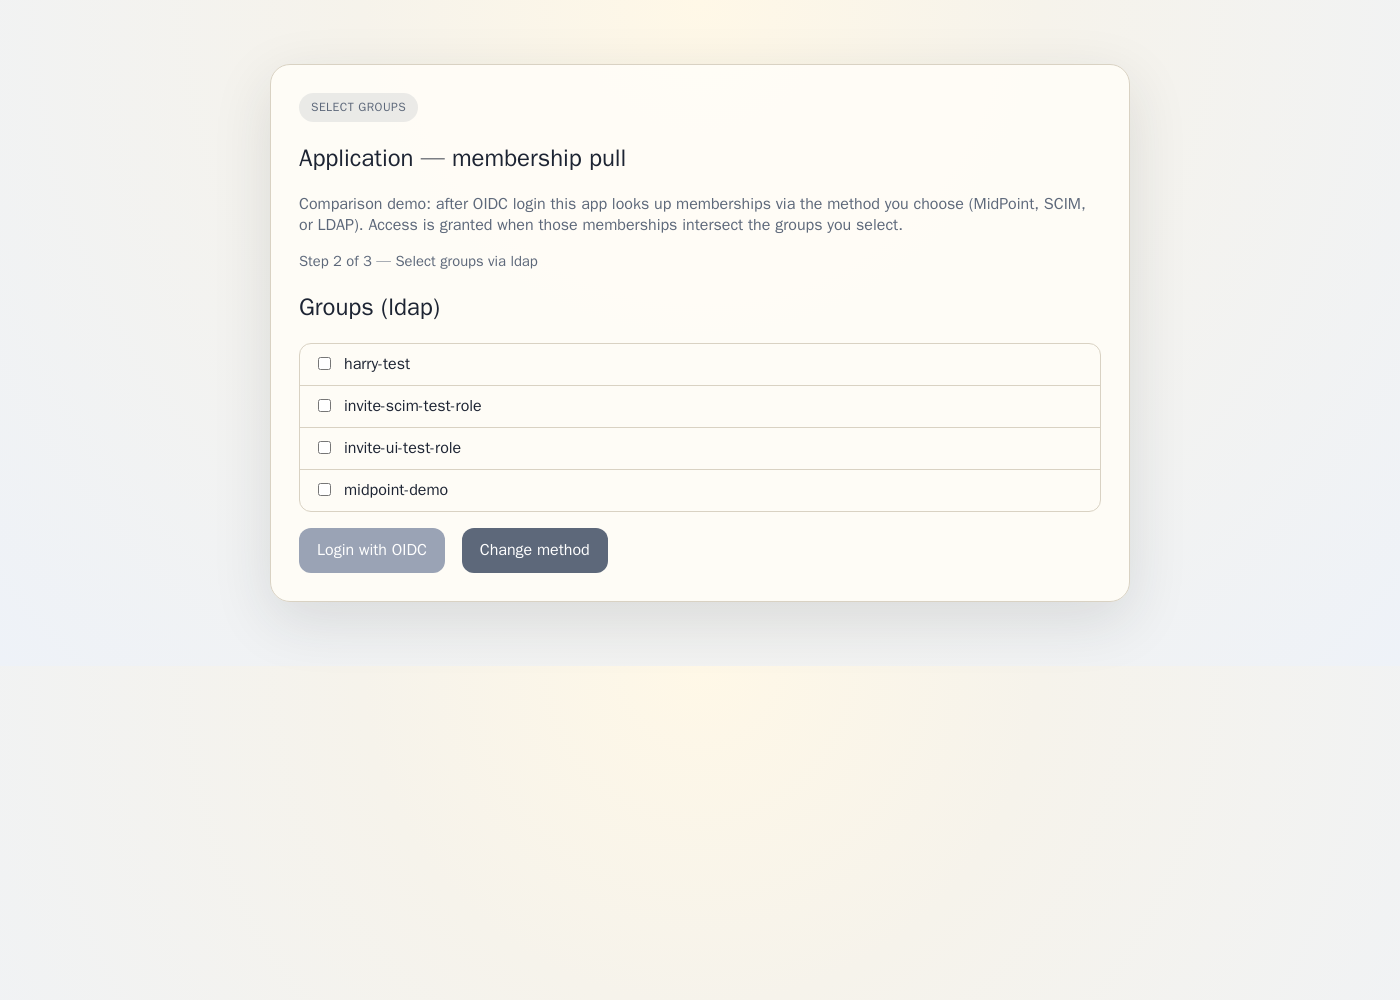
\includegraphics[width=0.92\textwidth]{figures/app-groups.png}
\caption{Application --- Step 2: groups discovered from the selected backend.}
\label{fig:app-groups}
\end{figure}

\begin{figure}[H]
\centering
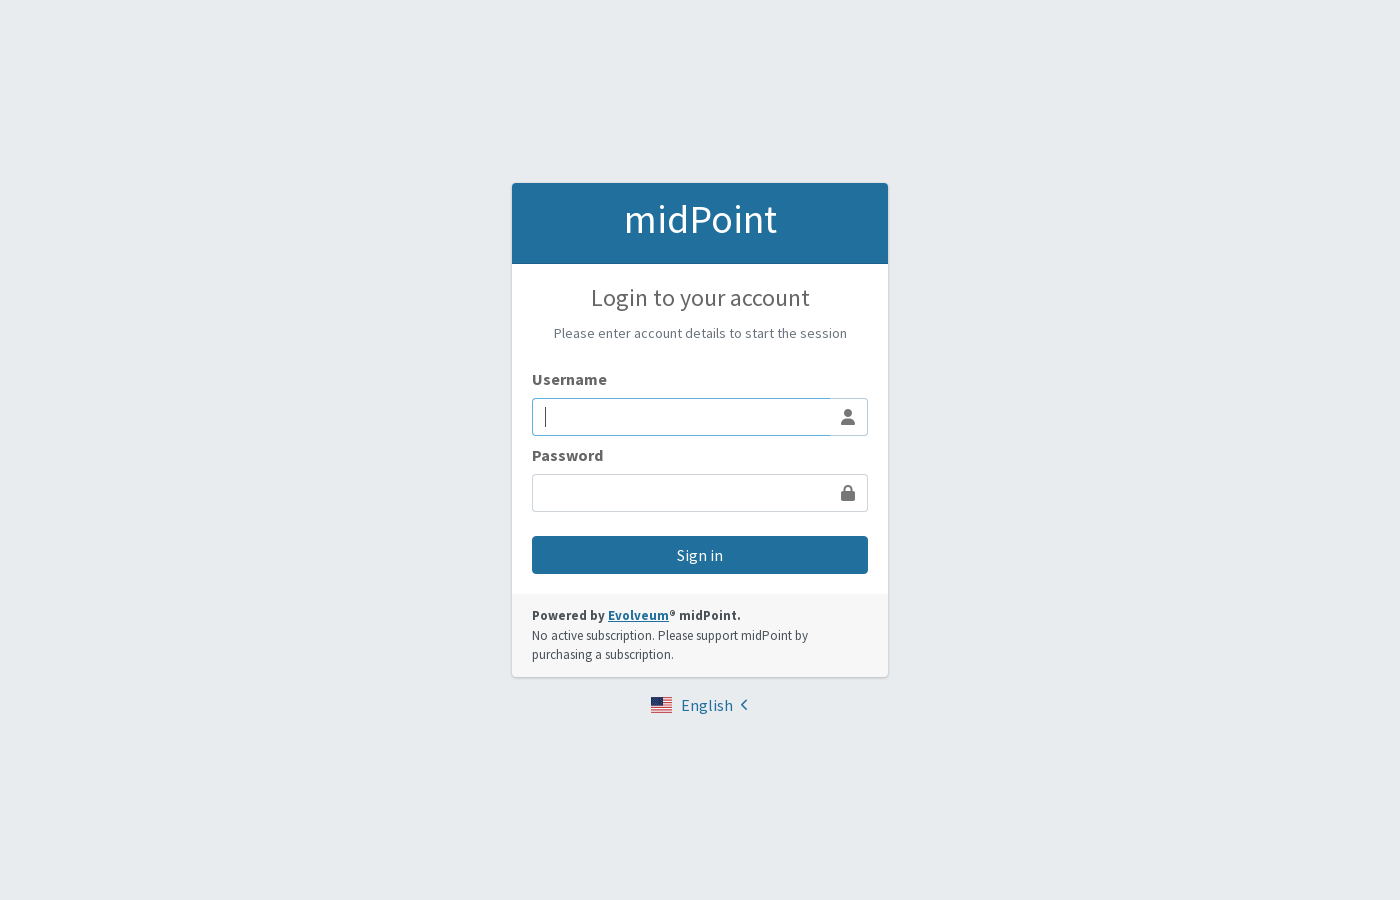
\includegraphics[width=0.72\textwidth]{figures/midpoint-login.png}
\caption{MidPoint GUI login at \host{midpoint.\$DOMAIN/midpoint/login}.}
\label{fig:midpoint-login}
\end{figure}

\subsection{Health endpoint}

\texttt{GET /health} reports backend readiness. Example from the running pilot:

\lstinputlisting[language={}]{figures/app-health.json}

% =============================================================================
\section{Deployment and configuration}
% =============================================================================

\subsection{Start the stack}

\begin{lstlisting}
# with Traefik (default Makefile target)
make build
# or
docker compose -f compose.yml -f compose.traefik.yml up -d --build

# Toggle Invite/OIDC profile via ENV_FILE=.env.invite | .test.env in .env
# then recreate invite_bridge (+ application if OIDC differs)
\end{lstlisting}

\subsection{Important environment variables}

\begin{table}[H]
\centering
\begin{tabularx}{\textwidth}{@{}l X@{}}
\toprule
\textbf{Variable} & \textbf{Purpose} \\
\midrule
\texttt{DOMAIN} & Base DNS name for Traefik hosts \\
\texttt{ENV\_FILE} & Invite/OIDC profile (\texttt{.env.invite} or \texttt{.test.env}) \\
\texttt{MIDPOINT\_ADMIN\_INITIAL\_PASSWORD} & MidPoint administrator password \\
\texttt{INVITE\_*} & Invite external API + Manage application linkage \\
\texttt{INVITE\_BRIDGE\_SYNC\_MEMBERSHIPS} & MidPoint unassign $\rightarrow$ Invite notify (default true) \\
\texttt{INVITE\_BRIDGE\_PUBLIC\_URL} & Target of MidPoint \textbf{Invite user} menu link \\
\texttt{INVITE\_BRIDGE\_UI\_PASSWORD} & HTTP Basic password for the invite form \\
\texttt{OIDC\_*} / \texttt{USER\_LOOKUP\_CLAIMS} & Demo app SURFconext RP (from profile) \\
\texttt{SCIM\_API\_KEY} & Bearer token for Invite $\rightarrow$ SCIM \\
\texttt{MIDPOINT\_LEADING\_GROUPS} & SCIM Group echo matches existing MidPoint Roles \\
\texttt{SCIM\_IDEMPOTENT\_USER\_CREATE} & Re-POST User reuses existing (avoids 409) \\
\bottomrule
\end{tabularx}
\caption{Key configuration knobs (see \texttt{.env.example} and profile files).}
\end{table}

\subsection{Traefik hostnames}

Assuming \texttt{DOMAIN=pilot1.sram.surf.nl}:

\begin{itemize}[leftmargin=*]
  \item Application: \url{https://app.pilot1.sram.surf.nl/}
  \item MidPoint: \url{https://midpoint.pilot1.sram.surf.nl/midpoint/}
  \item SCIM: \url{https://scim.pilot1.sram.surf.nl/}
  \item Invite user form: \url{https://invite-bridge.pilot1.sram.surf.nl/invite}
\end{itemize}

Configure the SURF Invite SCIM provisioner as described in
Section~\ref{sec:invite-provisioner} (Figure~\ref{fig:manage-provisioner}),
and configure \texttt{INVITE\_*} for \texttt{invite\_bridge} (see repository
\texttt{README.md}). Invite must use remote Manage so application metadata and
SCIM provisioners resolve correctly.

% =============================================================================
\section{Operational notes and lessons learned}
% =============================================================================

\begin{itemize}[leftmargin=*]
  \item \textbf{MidPoint owns Roles; Invite owns invitations.}
        \texttt{invite\_bridge} syncs Role create/delete to Invite; SCIM carries
        Users and memberships back into MidPoint. MidPoint \textbf{Invite user}
        only creates Invite invitations (roles must already have
        \texttt{scimResource}).
  \item \textbf{Drift prevention on MidPoint unassign.}
        Invite-SCIM memberships removed in MidPoint are notified to Invite via
        \texttt{by\_provisioned\_scim}. Local MidPoint revoke always wins if
        Invite notify fails.
  \item \textbf{Invite Manage must be remote.} If
        \texttt{/api/external/v1/manage/providers} only lists seed apps, Invite
        is on LocalManage---Roles show as ``unknown in Manage'' and SCIM may not
        fire.
  \item \textbf{\texttt{INVITE\_APPLICATION\_MANAGE\_TYPE}} must be uppercase
        (\texttt{SAML20\_SP}, \texttt{OIDC10\_RP}, \ldots).
  \item \textbf{\texttt{MIDPOINT\_LEADING\_GROUPS}.} Prevents Invite Group echoes
        from creating duplicate MidPoint Roles or deleting Roles on Group DELETE.
  \item \textbf{\texttt{SCIM\_IDEMPOTENT\_USER\_CREATE}.} Invite may re-POST an
        existing guest; reuse avoids 409 and broken accept flows.
  \item \textbf{Lookup key alignment.} Application
        \texttt{USER\_LOOKUP\_CLAIMS} must match the MidPoint user
        \texttt{name} written by SCIM (often the eduID EPPN).
\end{itemize}

% =============================================================================
\section{Parked components (not in default compose)}
\label{sec:parked}
% =============================================================================

The following remain in the repository for experiments but are \textbf{not}
started by \texttt{compose.yml}:

\begin{itemize}[leftmargin=*]
  \item OpenLDAP / phpLDAPadmin / MidPoint OpenLDAP resource and
        \texttt{metarole-ldap-group} post-initial objects (\texttt{ldap/},
        \texttt{midpoint/post-initial-objects/100-*} / \texttt{110-*}).
  \item Moodle / \texttt{moodle\_bridge} / ConnId Moodle resource.
  \item OneRoster / NRPS LMS path.
\end{itemize}

See repository \texttt{TODO.md}.

% =============================================================================
\section{Summary}
% =============================================================================

The stack demonstrates a MidPoint-leading Invite path:

\begin{center}
\textbf{MidPoint $\xrightarrow{\texttt{invite\_bridge}}$ Invite $\xrightarrow{\mathrm{SCIM}}$ MidPoint}\\[0.4em]
\small (+ MidPoint membership revoke $\rightarrow$ Invite \texttt{by\_provisioned\_scim};\\
optional OIDC app membership pull)
\end{center}

Roles created in MidPoint appear in Invite for invitation workflows; administrators
can start invitations from MidPoint's \textbf{Invite user} menu or from Invite
itself; accepted guests are provisioned as MidPoint users with role assignments
via SCIM; MidPoint unassigns of Invite-SCIM members notify Invite to prevent
drift. Reusable custom pieces for other MidPoint installations are
\texttt{invite\_bridge} and the SCIM MidPoint plugin leading-mode behaviour.

\appendix
\section{Quick reference commands}

\begin{lstlisting}
# Follow MidPoint -> Invite sync / revoke notify
docker compose -f compose.yml -f compose.traefik.yml logs -f invite_bridge

# Follow SCIM (Users/memberships and Group echoes)
docker compose -f compose.yml -f compose.traefik.yml logs -f scim

# Unit tests
cd invite_bridge && python -m unittest test_membership_sync.py -v

# Manual Invite role create
./scripts/invite-create-role.sh my-role-name

# Application health
curl -s https://app.$DOMAIN/health | jq .
\end{lstlisting}

\end{document}
